\begin{abstract}
Audio language models now grade spoken answers, on the assumption that they score what was said and not how it sounded. We test this by holding the words fixed and changing only the voice. With one text-to-speech (TTS) voice per gender (192 clips), Gemini 3.1 Pro scores Indian-accented answers 2.50 points lower than identical American-accented ones on a 100-point scale ($p=0.005$), Gemini 3.6 Flash does not ($-0.04$), and Qwen2-Audio-7B scores non-American accents 2 to 3 points higher. Grading the judge's own transcript removes Pro's penalty (interaction $-6.04$, $p=4\times10^{-4}$). Six more voices dissolve it: Pro's Indian shift becomes $-0.76$ ($p=0.35$), with single voices ranging from $+2.08$ to $-4.58$. On real speech (24 L2-ARCTIC speakers, six first languages, 240 clips), both Gemini judges penalise every non-native language by 4 to 16 points (all $p\le4\times10^{-4}$), while Qwen2-Audio barely moves. One voice per accent, the common audit design, produced a significant bias finding that did not replicate.
\end{abstract}

\begin{figure}[t]
\centering
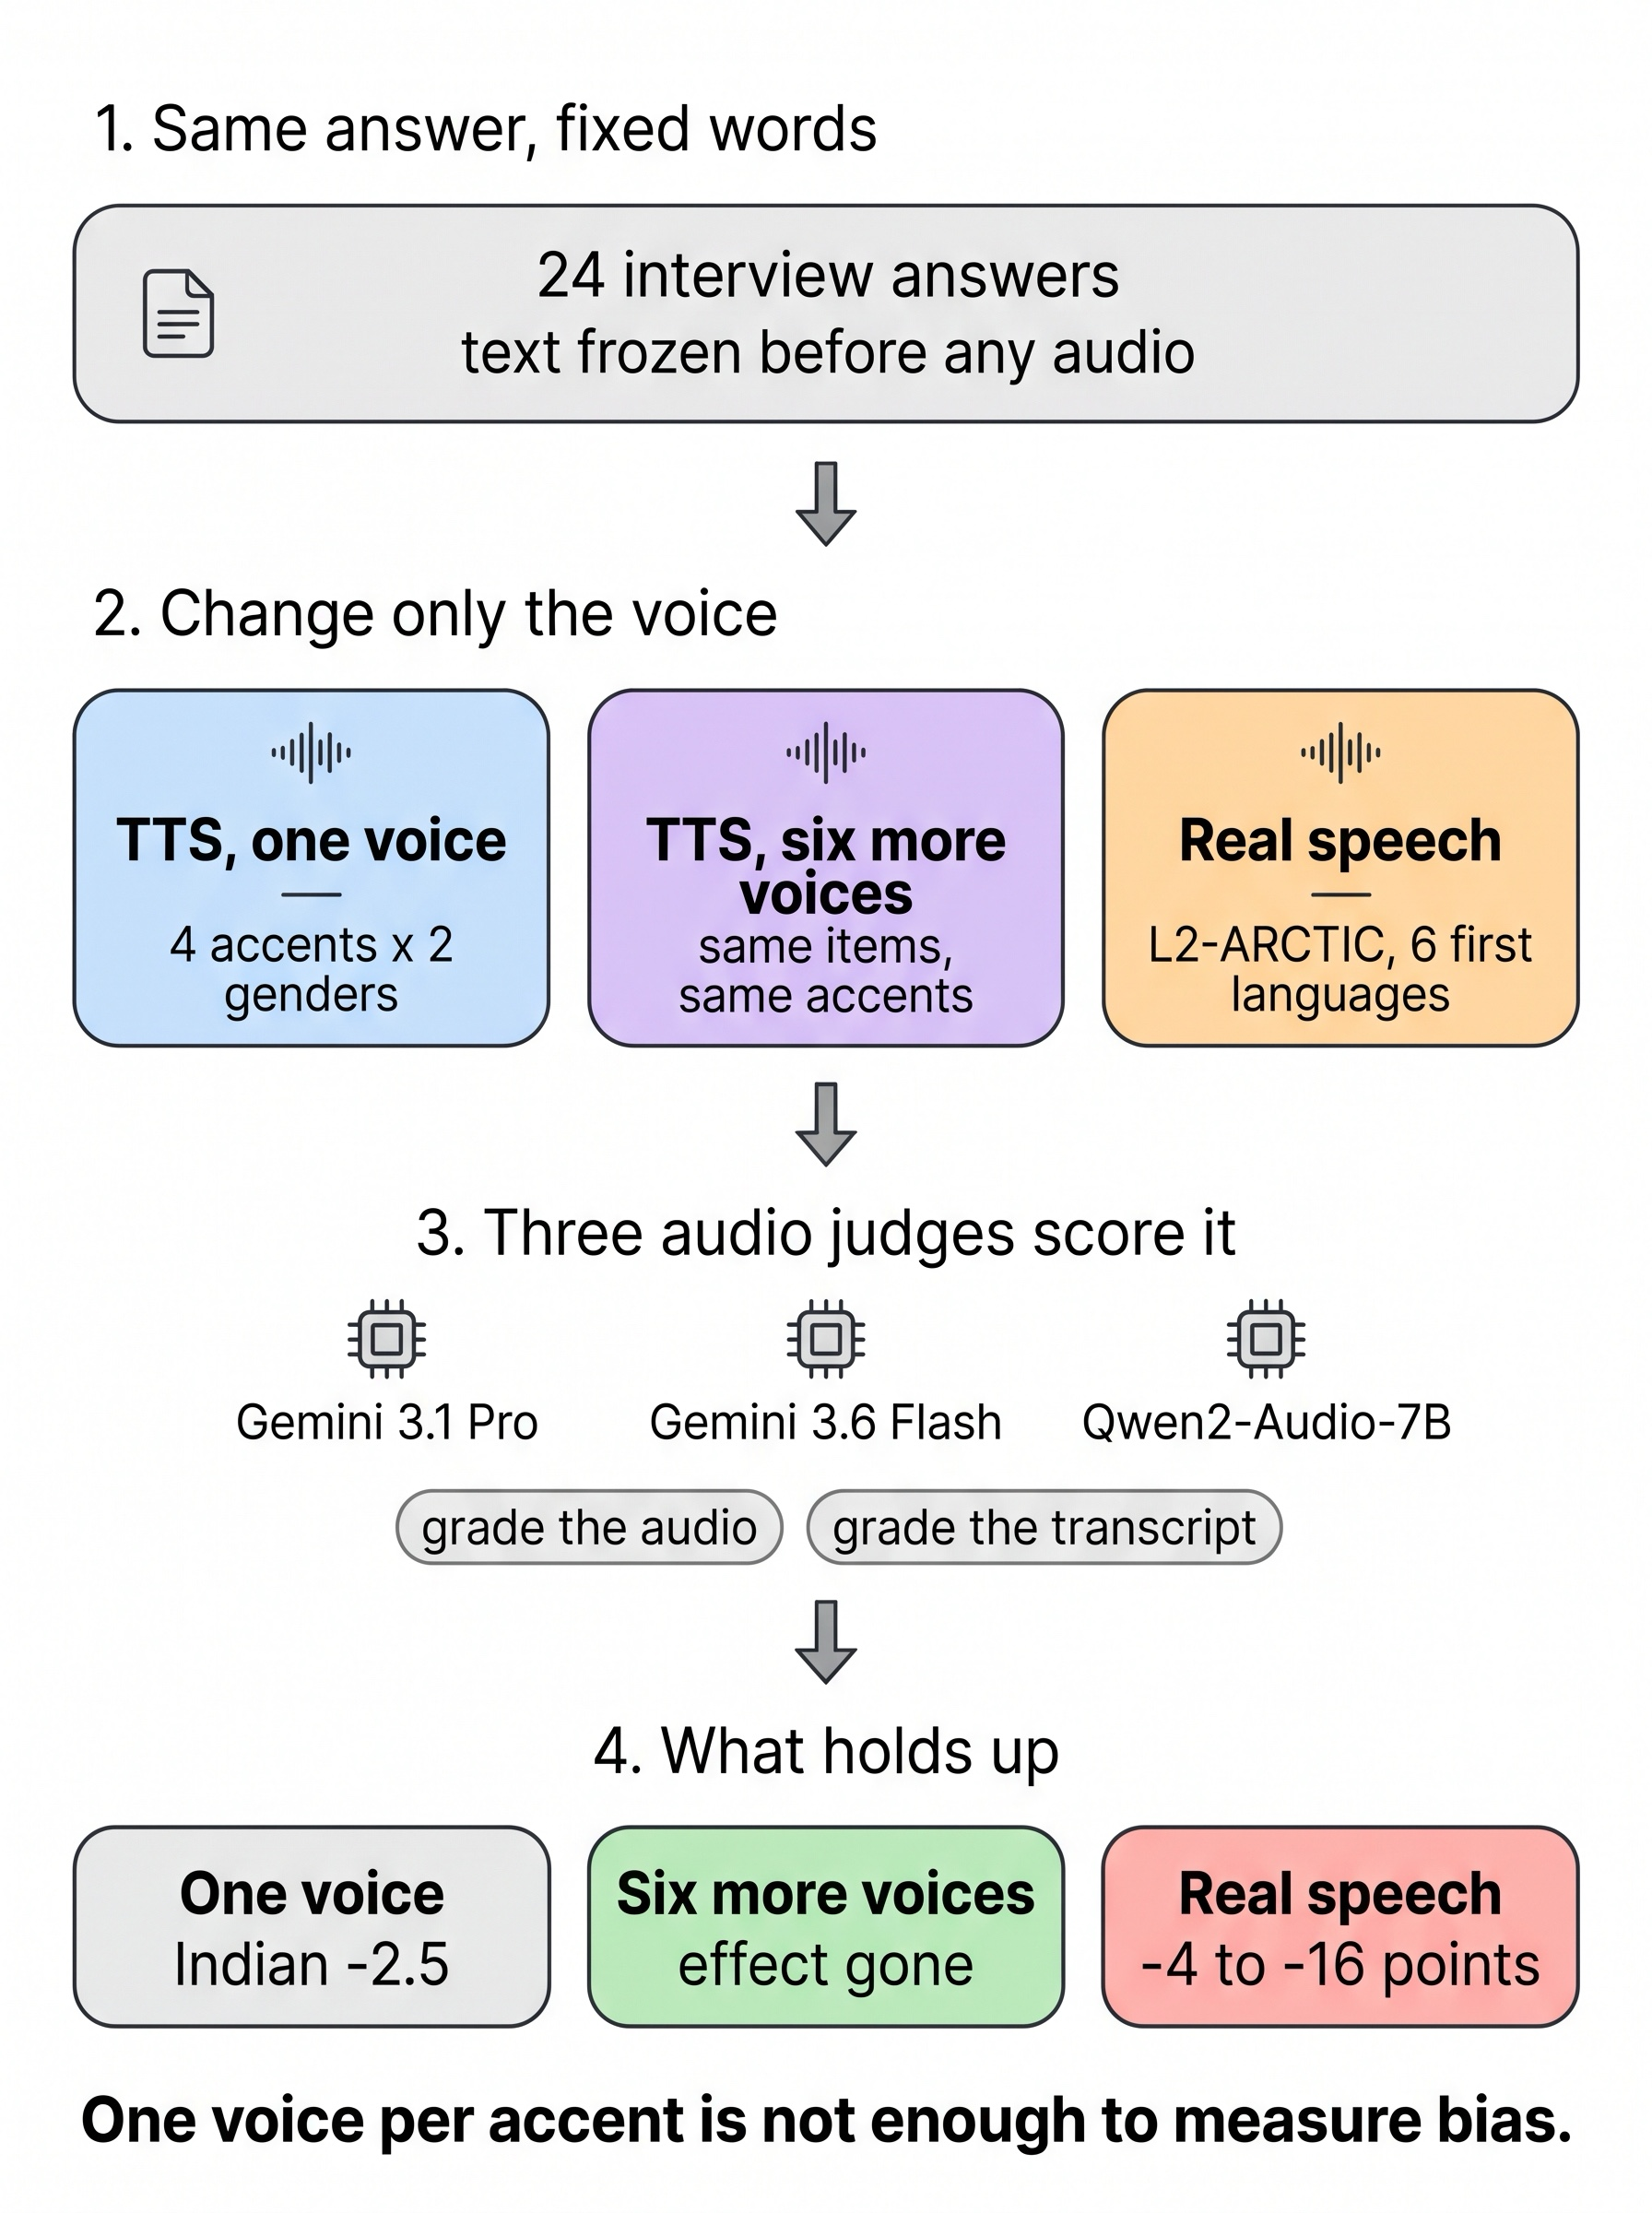
\includegraphics[width=0.86\columnwidth]{assets/fig1_schematic.jpg}
\caption{Study design. (1) 24 interview answers are written once and frozen. (2) Only the voice changes: one TTS voice pair in four accents, six further TTS voices, and real non-native speakers. (3) Three audio judges score each clip, and the Gemini judges also grade transcripts of the same audio. (4) The single-voice penalty disappears with more voices, while real speech shows large penalties. Schematic generated with Nano Banana 2 and checked by hand; numbers are from Tables~\ref{tab:axisa}--\ref{tab:l2arctic}.}
\label{fig:schematic}
\end{figure}

\section{Introduction}
\label{sec:intro}

An audio language model that grades a spoken answer has to do two things: understand the content and ignore the voice that carries it. Several kinds of systems already rely on the second part. Speech LLMs are being trained to grade the oral proficiency of second-language (L2) speakers, who bring a wide range of accents \citep{ma2025assessmentof}. AI interview systems run at scale: one study samples from over 300,000 AI-conducted job interviews and evaluates them with an LLM judge \citep{allbert2025evaluatingsp}, and earlier work catalogued sources of bias in automated video interviews \citep{booth2023integratingp}. Audio models are also used as judges to rank speech systems \citep{manakul2025audiojudgeun}. If the judge's score moves with the speaker's voice, these systems are partly scoring the speaker.

Prior work has studied the pieces of this question separately. Audio judges have been built and validated for speech quality, speaking style and paralinguistic cues \citep{manakul2025audiojudgeun,wang2025speechllmasj,chiang2025audioawarela,jeon2026parapairaudi}, and audited for protocol shortcuts \citep{park2026auditingprot} and for whether they use paralinguistic evidence at all \citep{miller2026doaudiolangu}. Voice bias has been measured when the speech model is the respondent: its reply changes with the asker's accent or gender \citep{satish2026thevoicebehi,lin2026vibevoiceind,wu2025evaluatingbi}, or its answer to a spoken multiple-choice question changes with the voice \citep{wei2026biasintheear}. Fairness has been studied in L2 speaking graders through their internal representations \citep{labroo2026biasanalysis} and in speech recognition across speaker groups \citep{koenecke2020racial,ginjala2026doLLMdecoders}.

\textbf{The gap.} None of these studies puts an audio model in the grader role, holds the evaluee's words fixed, and treats the evaluee's voice as the experimental variable. Most voice-bias studies also build their conditions with one synthetic voice per accent or gender. That design confounds the accent with everything else the chosen voice carries, and nobody has checked whether a finding from it survives a change of voice.

We ran that test and then tried to replicate our own result. Our contributions are:
\begin{enumerate}
\item \textbf{A three-arm audit of audio judges.} Single-voice TTS, multi-voice TTS and real speech, scored by three judges from two families, with the words held fixed in every comparison (Section~\ref{sec:setup}).
\item \textbf{A replication failure in the common design.} The single-voice arm produced a significant Indian-accent penalty under Gemini 3.1 Pro ($-2.50$, $p=0.005$) that survives correction. With six more voices it falls to $-0.76$ ($p=0.35$), and under a four-part rubric to $-0.33$ (Section~\ref{sec:multivoice}).
\item \textbf{A channel test.} For the original voice pair, grading the judge's own transcript removes the penalty (interaction $-6.04$, $p=4\times10^{-4}$), so it lives in the audio and not in the recognised words (Section~\ref{sec:decomp}).
\item \textbf{Large, consistent penalties on real speech.} On L2-ARCTIC, both Gemini judges penalise all six non-native first languages, by 4 to 16 points, with the same ordering, while Qwen2-Audio barely moves (Section~\ref{sec:realspeech}).
\item \textbf{A comparison with prior voice-bias results.} We place our three arms next to published studies of audio models as respondents, test-takers, graders and transcribers (Section~\ref{sec:prior}).
\end{enumerate}

\section{Related Work}
\label{sec:related}

\textbf{Audio models as judges.} AudioJudge shows that large audio models can judge speech and reports verbosity and position biases in that role \citep{manakul2025audiojudgeun}. Judge-construction work trains or prompts audio models to rate speech quality and speaking style \citep{wang2025speechllmasj,zhang2026jastinaligni,chen2025audiolargela,chiang2025audioawarela}. ParaPairAudioBench tests whether an audio judge detects paralinguistic differences in same-transcript and cross-transcript pairs \citep{jeon2026parapairaudi}. Counterfactual audits hold a transcript fixed and vary affect or prosody to check whether a judge uses the audio cue \citep{miller2026doaudiolangu}, and protocol audits show that judges can take shortcuts through labels or reference data instead of listening \citep{park2026auditingprot}. These studies vary the delivery the judge should notice. We vary the speaker identity the judge should ignore.

\textbf{Voice bias in speech models as respondents.} The Voice Behind the Words varies the accent and gender of the person asking a question across 2,880 interactions, keeping content fixed through voice cloning, and finds lower helpfulness scores for Eastern European accents, especially for female voices \citep{satish2026thevoicebehi}. A companion study repeats this with judge-free metrics and a user study \citep{satish2026fromseeingit}. VIBE uses human-recorded speech in open-ended tasks and finds that gender and accent cues shift model outputs \citep{lin2026vibevoiceind}. Spoken-dialogue and speech-continuation studies find similar effects for age, gender, accent and phonation type \citep{wu2025evaluatingbi,satish2025speakyourmin,choi2025acousticbase}, and a fine-tuning study shows that results from multiple-choice bias benchmarks do not carry over to long-form tasks \citep{satish2025dobiasbenchm}. BiasInEar varies the voice of a spoken multiple-choice question and finds models fairly robust to demographic factors but sensitive to language and option order \citep{wei2026biasintheear}. VocalBench-DF tests robustness to disfluent speech \citep{liu2025vocalbenchdf}. In all of these the model answers. In ours it grades.

\textbf{Fairness in speech assessment and recognition.} Automatic L2 speaking graders have been probed for encoded speaker attributes with concept activation vectors \citep{labroo2026biasanalysis}, and a hybrid L2 speaking scorer has been benchmarked against the agreement of trained human raters \citep{uehara2026interpretabl}. LLM pronunciation feedback on L2-ARCTIC often gives coherent reasoning for a wrong rating \citep{wang2026priorongevidence}. Commercial speech recognisers have nearly twice the word error rate for Black speakers as for white speakers \citep{koenecke2020racial}, and Whisper hallucinates far more on Indian-accented speech than LLM-decoder recognisers do \citep{ginjala2026doLLMdecoders}. Human quality ratings carry gender bias \citep{ren2026mosbiasfromh}, and automatic quality predictors miss prosodic errors that listeners hear \citep{takagi2026investigatin}. Before audio models, listeners were shown to evaluate the same speech differently once they believed the speaker belonged to a different group \citep{kang2009reverse}. That is the causal logic we apply to an artificial judge.

\textbf{TTS as an experimental instrument.} Accent similarity in synthesis is hard to evaluate \citep{zhong2025pairwiseeval}, a listening benchmark of codec and TTS speech across ten accents finds that listeners rate speakers of their own accent differently \citep{huang2026codecmosacce}, scaling accented TTS needs automatic accent-label discovery and voice augmentation \citep{xinyuan2025scalablecont}, and current TTS evaluation is argued to miss broader effects \citep{yang2025positiontowa}. Our multi-voice result gives direct evidence for this concern about using TTS voices as stand-ins for groups of speakers.

\section{Experimental Setup}
\label{sec:setup}

\subsection{Answer Bank}
We wrote 24 interview-style question-and-answer pairs across ten everyday domains with a text model (Gemini 3.5 Flash), aiming at medium quality so a judge has room to move the score. A first version was too good: answers meant to be ``incomplete or shallow'' scored a mean of 94.3 out of 100 under an audio judge. A rewritten prompt that required checkable weaknesses produced a bank with mean 61.3 (sd 17.0, range 20 to 90) under Gemini 3.6 Flash, which we froze and used throughout.

\subsection{Voice Conditions}
\textbf{Single-voice TTS arm.} Each answer was rendered with Gemini 3.1 Flash TTS in four accents (American, British, Indian and Nigerian English) and two genders, one prebuilt voice per gender (Charon and Kore), giving 192 clips. The accent was set by a natural-language style instruction. Before generation, a blind classifier identified the intended accent and gender in 8 of 8 pilot clips.

\textbf{Multi-voice replication.} Because one voice per cell mixes accent with everything else that voice carries, we re-rendered a 12-item subset in all four accents with six more voices (Puck, Fenrir and Orus; Aoede, Leda and Zephyr), giving 288 clips. Separately, we re-scored the original 192 clips with a decomposed rubric: correctness, completeness, helpfulness and clarity, 0 to 25 each.

\textbf{Real speech.} L2-ARCTIC \citep{zhao2018l2arctic} has 24 non-native English speakers, two women and two men for each of six first languages (Arabic, Hindi, Korean, Mandarin, Spanish and Vietnamese), who read the same prompt sentences as the native CMU ARCTIC voices. We chose eight sentences recorded by all 24 L2 speakers and six native voices (bdl, rms, jmk, awb; slt, clb), giving 240 clips. ARCTIC sentences are generic prompts rather than answers, so this arm uses a read-aloud rubric that scores clarity, fluency and how professional the reading sounds. It measures how strongly a judge responds to non-native speech, not content bias.

\textbf{Delivery perturbations.} With one voice (American, female) we made five versions of each answer: filled pauses, slowed ($0.85\times$) and sped up ($1.25\times$) speech, an 8 kHz telephone channel, and pink noise at 10 dB SNR. A clip was kept only if its word error rate against the frozen text was at most 5\%. Five of 120 conditions failed and were dropped, leaving 139 clips including the clean originals. Each was scored under a neutral rubric and under an instruction to ignore delivery.

All clips were loudness-normalised with the same \texttt{ffmpeg loudnorm} recipe and resampled to 16 kHz.

\subsection{Judges and Protocol}
Table~\ref{tab:setup} lists the judges and what each scored. The Gemini judges were called through the API at temperature 0, one clip per call, in random order, and were never told the study concerns voice. Qwen2-Audio-7B-Instruct ran on one A10G GPU with greedy decoding. The content rubric asks for one 0 to 100 score covering correctness, completeness, helpfulness and clarity, plus a one-sentence reason, as JSON. For the channel test, each Gemini judge also transcribed the audio and graded its own transcript, and graded the frozen gold text. Prompts are in Appendix~\ref{app:prompts}.

\begin{table}[t]
\small
\centering
\setlength{\tabcolsep}{3pt}
\begin{tabular}{lccc}
\toprule
Arm (clips) & Pro & Flash & Qwen2-Audio \\
\midrule
Single-voice TTS (192) & \checkmark & \checkmark & \checkmark \\
Multi-voice TTS (288) & \checkmark & \checkmark & -- \\
Decomposed rubric (192) & \checkmark & -- & -- \\
Transcript grading (24 pairs) & \checkmark & \checkmark & -- \\
Delivery perturbations (139) & \checkmark & \checkmark & -- \\
Real speech, L2-ARCTIC (240) & \checkmark & \checkmark & \checkmark \\
\bottomrule
\end{tabular}
\caption{Judges and arms. Pro = Gemini 3.1 Pro (API), Flash = Gemini 3.6 Flash (API), Qwen2-Audio = Qwen2-Audio-7B-Instruct (open weights, local GPU).}
\label{tab:setup}
\end{table}

\subsection{Statistical Analysis}
The unit of analysis is the item. For item $i$ and condition $c$ we form the paired difference $\Delta_i = s_i^{c} - s_i^{\mathrm{ref}}$, where the reference is the gender-matched American rendering in the TTS arms and the gender-matched native mean in the real-speech arm. We report the mean $\bar{\Delta}$ with a 95\% percentile bootstrap interval from 10{,}000 resamples \citep{efron1979}, a two-sided sign-flip permutation test with 20{,}000 permutations \citep{good2005}, and the paired effect size $d_z = \bar{\Delta}/s_\Delta$ \citep{lakens2013}. The channel test compares grading modes on the same items with a difference of differences, $(\Delta^{\text{audio}}_i - \Delta^{\text{transcript}}_i)$, tested the same way. All 33 accent-by-judge-by-arm tests form one Benjamini-Hochberg family at $q=0.05$ \citep{bh1995}. Every number comes from scripted analyses of the raw logs.

\textbf{Pre-registration.} Four directions were written in the project log before any data was collected: D1, judges score L2 and Global South accents lower for identical words; D2, sign and size differ across judge families; D3, transcript grading removes most of the acoustic effect; D4, delivery perturbations shift content scores despite an instruction to ignore delivery.

\section{Results}
\label{sec:results}

\subsection{The Single-Voice Arm Shows an Accent Penalty}
\label{sec:singlevoice}

Table~\ref{tab:axisa} and Figure~\ref{fig:forest} give the single-voice results. Gemini 3.1 Pro scores Indian-accented answers 2.50 points below the identical American-accented answers ($p=0.005$, $d_z=-0.44$). The same comparison under Gemini 3.6 Flash is $-0.04$ ($p=1.0$). Qwen2-Audio moves the other way and scores every non-American accent higher: British $+2.92$ ($p=0.011$), Indian $+1.98$ ($p=0.044$) and Nigerian $+2.29$ ($p=0.014$). Its scores take only four distinct values between 75 and 95, so its shifts are coarse. Gender has no significant effect under either Gemini judge (Flash $+3.25$ toward the female voice, $p=0.12$; Pro $-0.83$, $p=0.47$). On its own, this arm suggests a judge-specific accent penalty.

\begin{table}[t]
\small
\centering
\setlength{\tabcolsep}{4pt}
\begin{tabular}{llrcr}
\toprule
Judge & Accent & Shift & 95\% CI & $p$ \\
\midrule
Pro & British & $-0.42$ & [$-2.08$, $+1.25$] & 0.73 \\
 & Indian & $\mathbf{-2.50}$ & [$-4.06$, $-0.94$] & \textbf{0.005} \\
 & Nigerian & $+1.04$ & [$-0.52$, $+2.60$] & 0.26 \\
\midrule
Flash & British & $-1.08$ & [$-3.90$, $+1.92$] & 0.49 \\
 & Indian & $-0.04$ & [$-2.85$, $+2.73$] & 1.00 \\
 & Nigerian & $+0.23$ & [$-2.60$, $+3.08$] & 0.89 \\
\midrule
Qwen & British & $\mathbf{+2.92}$ & [$+0.94$, $+5.00$] & \textbf{0.011} \\
 & Indian & $+1.98$ & [$+0.21$, $+3.75$] & 0.044 \\
 & Nigerian & $\mathbf{+2.29}$ & [$+0.73$, $+4.06$] & \textbf{0.014} \\
\bottomrule
\end{tabular}
\caption{Single-voice TTS arm: score shift against the gender-matched American rendering, $n=48$ pairs per cell. Bold: survives Benjamini-Hochberg over all 33 accent tests.}
\label{tab:axisa}
\end{table}

\begin{figure}[t]
\centering
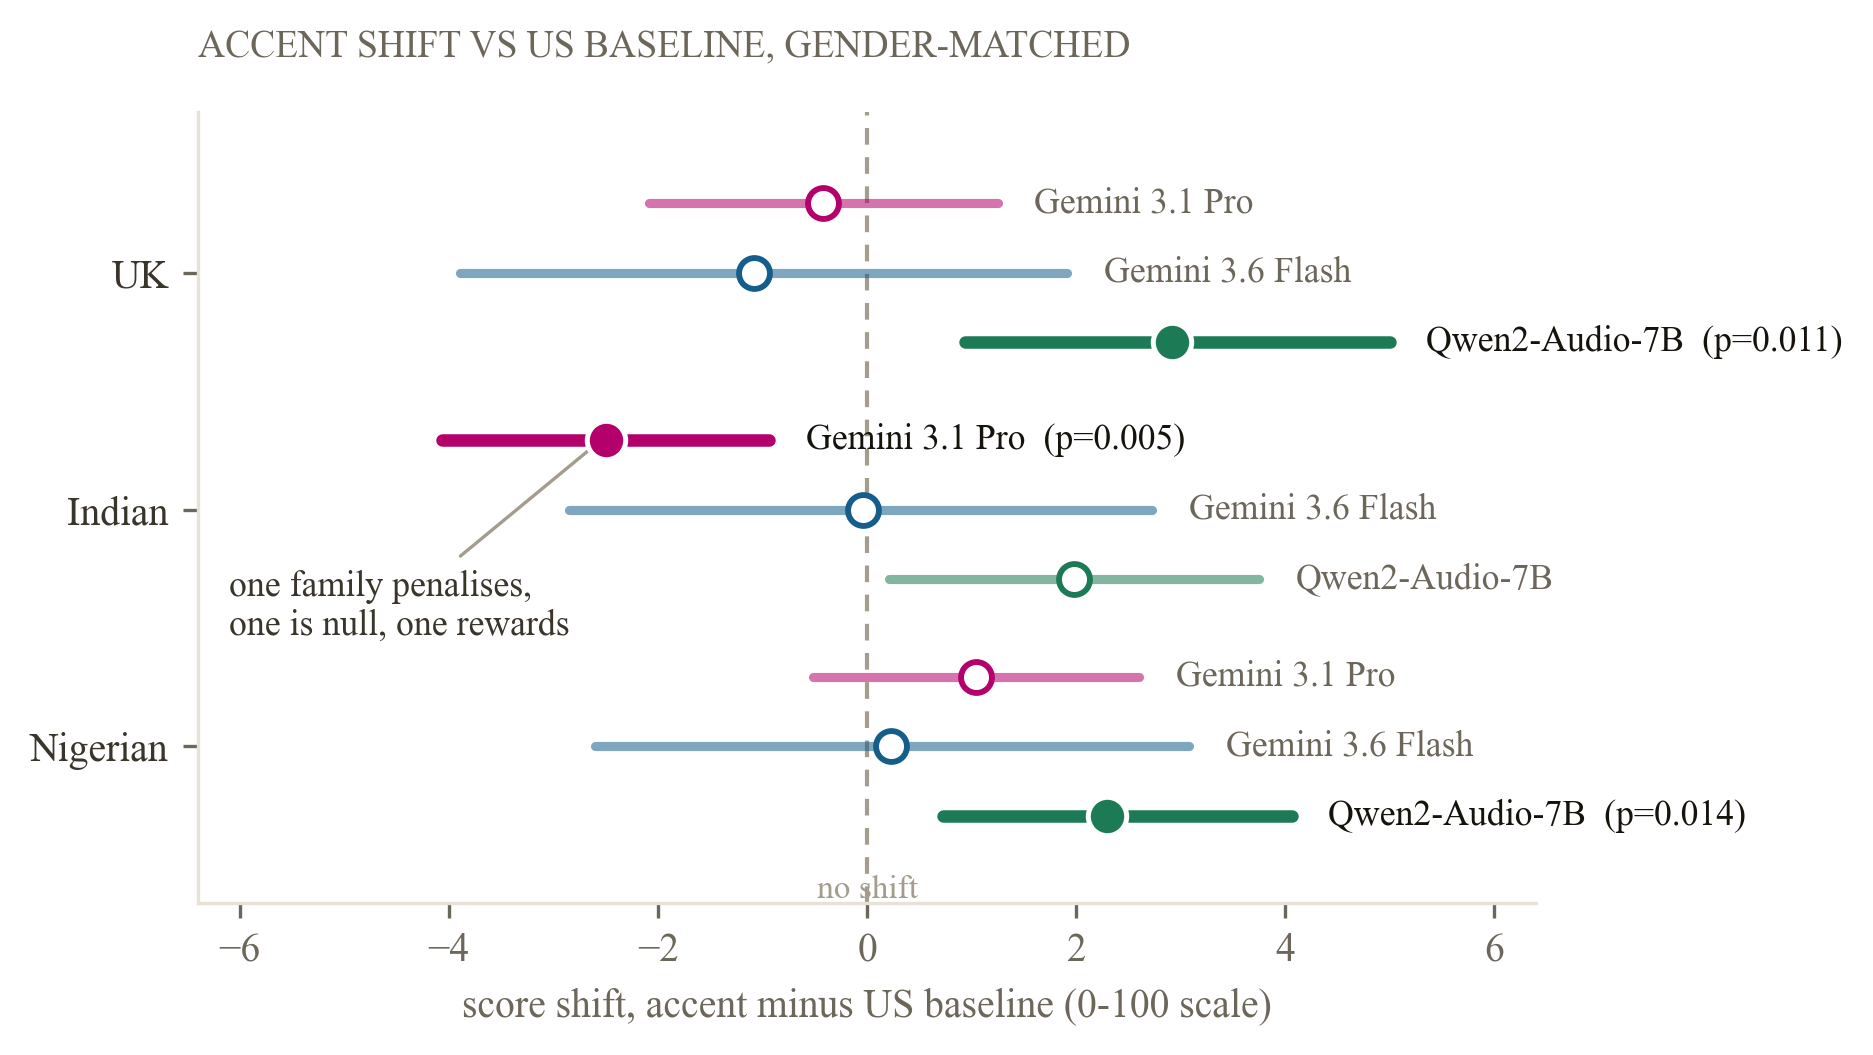
\includegraphics[width=\columnwidth]{assets/figure1_accent_forest.png}
\caption{Single-voice TTS arm: score shift by accent and judge with 95\% bootstrap intervals, $n=48$ per interval. Right of the dashed line means the accent scored higher than American. Filled markers survive correction.}
\label{fig:forest}
\end{figure}

\subsection{The Penalty Does Not Replicate}
\label{sec:multivoice}

\textbf{Six more voices.} With six new voices reading the same items in the same accents (Tables~\ref{tab:multivoice} and \ref{tab:pervoice}, Figure~\ref{fig:multivoice}), Pro's Indian shift is $-0.76$ (CI $[-2.22, +0.69]$, $p=0.35$, $n=72$). The individual voices range from $+2.08$ (Fenrir) to $-4.58$ (Zephyr), and the original pair's $-2.50$ falls inside that range. The voice moves the score more than the accent does. Flash is just as unstable: its Indian shift is $+0.11$ ($p=0.95$) with per-voice means from $-2.67$ to $+4.17$, and its Nigerian shift is significantly negative ($-3.22$, $p=0.0042$) where the single-voice arm showed a slight positive trend.

\textbf{A different rubric.} Re-scoring (Table~\ref{tab:dims}) the original 192 clips with the four-part rubric, Pro's Indian shift is $-0.15$ for correctness ($p=0.66$), $-0.17$ for completeness ($p=0.56$), $+0.21$ for helpfulness ($p=0.46$) and $-0.23$ for clarity ($p=0.48$), or $-0.33$ in total on the 100-point scale ($n=48$). The same clips that give $-2.50$ under one holistic score give nothing under sub-scores.

The $-2.50$ cell survives correction even in the joint 33-test family. Correction controls false positives within a design, but it cannot detect a design that confounds the accent with one voice. Only replication shows that.

\begin{table}[t]
\small
\centering
\setlength{\tabcolsep}{4pt}
\begin{tabular}{llrcr}
\toprule
Judge & Accent & Shift & 95\% CI & $p$ \\
\midrule
Pro & British & $+0.90$ & [$-0.69$, $+2.57$] & 0.32 \\
 & Indian & $-0.76$ & [$-2.22$, $+0.69$] & 0.35 \\
 & Nigerian & $+1.53$ & [$+0.14$, $+2.92$] & 0.043 \\
\midrule
Flash & British & $-1.81$ & [$-4.03$, $+0.42$] & 0.12 \\
 & Indian & $+0.11$ & [$-2.11$, $+2.33$] & 0.95 \\
 & Nigerian & $\mathbf{-3.22}$ & [$-5.38$, $-1.14$] & \textbf{0.0042} \\
\bottomrule
\end{tabular}
\caption{Multi-voice replication: shift against the gender-matched American rendering across six new voices, $n=72$ pairs per cell (12 items $\times$ 6 voices). Bold: survives the joint correction.}
\label{tab:multivoice}
\end{table}

\begin{table}[t]
\small
\centering
\begin{tabular}{lrr}
\toprule
Voice & Gemini 3.1 Pro & Gemini 3.6 Flash \\
\midrule
Charon/Kore (original) & $-2.50$ & $-0.04$ \\
Aoede & $+1.67$ & $+1.67$ \\
Fenrir & $+2.08$ & $+4.17$ \\
Leda & $+0.83$ & $-2.67$ \\
Orus & $-2.08$ & $+1.67$ \\
Puck & $-2.50$ & $-2.50$ \\
Zephyr & $-4.58$ & $-1.67$ \\
\midrule
Six new voices, pooled & $-0.76$ & $+0.11$ \\
\bottomrule
\end{tabular}
\caption{Indian-minus-American shift per voice, $n=12$ item-gender pairs per voice (original pair $n=48$; pooled $n=72$).}
\label{tab:pervoice}
\end{table}

\begin{table}[t]
\small
\centering
\begin{tabular}{lrr}
\toprule
Dimension (0--25) & Shift & $p$ \\
\midrule
Correctness & $-0.15$ & 0.66 \\
Completeness & $-0.17$ & 0.56 \\
Helpfulness & $+0.21$ & 0.46 \\
Clarity & $-0.23$ & 0.48 \\
Total (0--100 equivalent) & $-0.33$ & 0.70 \\
\bottomrule
\end{tabular}
\caption{Gemini 3.1 Pro, original 192 clips re-scored with the decomposed rubric: Indian-minus-American shift per dimension, $n=48$ pairs. The holistic score's $-2.50$ has no counterpart in the sub-scores.}
\label{tab:dims}
\end{table}

\begin{figure}[t]
\centering
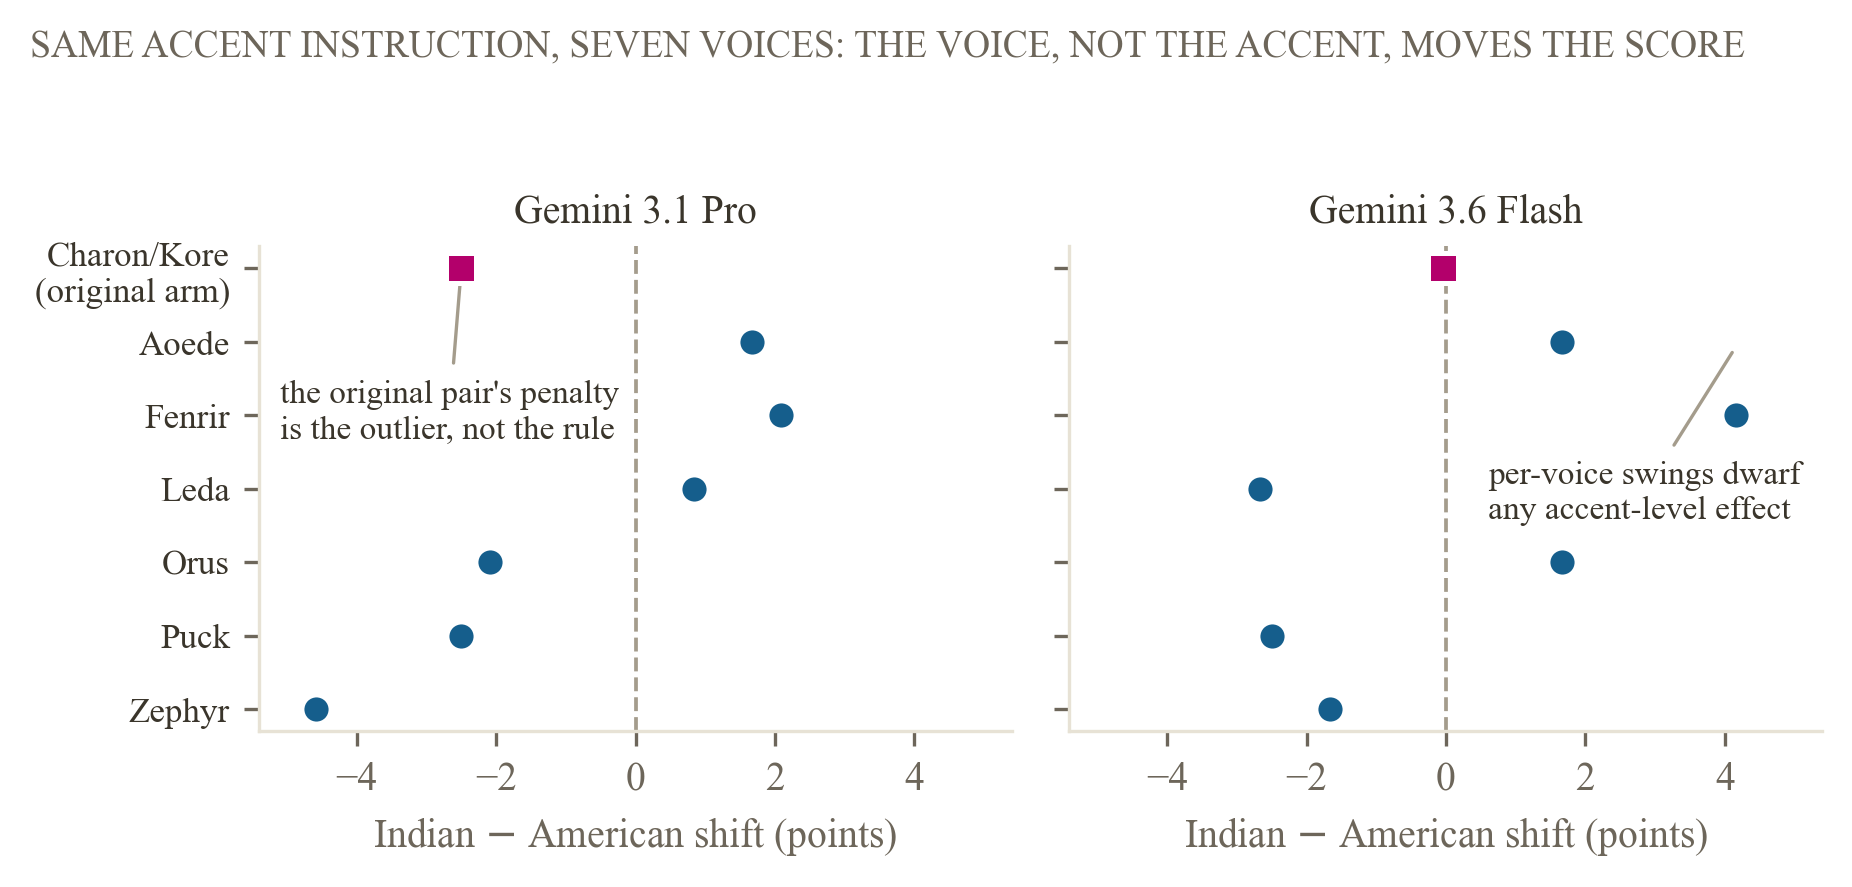
\includegraphics[width=\columnwidth]{assets/figure4_multivoice.png}
\caption{Indian-minus-American shift for each voice ($n=12$ pairs per voice; original pair $n=48$). The original pair's penalty lies inside the spread across voices.}
\label{fig:multivoice}
\end{figure}

\subsection{The Original Penalty Is in the Audio}
\label{sec:decomp}

For the original voice pair, where the penalty appeared, we graded the same answers three ways (Table~\ref{tab:decomp}, Figure~\ref{fig:decomp}). The Indian shift is $-2.50$ from audio, $+1.88$ from Pro's own transcript of that audio, and $-0.83$ from the gold transcript. Since a difference in significance is not itself a significant difference, we test the interaction directly. The audio shift differs from the own-transcript shift by $-6.04$ points (CI $[-8.54, -3.54]$, $p=4\times10^{-4}$, $n=24$) and from the gold-transcript shift by $-3.33$ ($[-5.83, -0.83]$, $p=0.028$). Whatever Pro penalises in this voice pair is in the sound and disappears once the speech is transcribed. The gold-transcript mode is only a sanity check, because identical text should get identical scores; the informative contrast is audio against the judge's own transcript. Flash has no audio effect to decompose and shows nothing in either transcript mode ($-4.25$, $p=0.17$; $+0.83$, $p=0.36$). Transcript-first grading is therefore a working mitigation, but it removes everything the audio carries, legitimate or not.

\begin{table}[t]
\small
\centering
\setlength{\tabcolsep}{4pt}
\begin{tabular}{lrcr}
\toprule
Grading mode & Shift & 95\% CI & $p$ \\
\midrule
Audio & $-2.50$ & [$-4.06$, $-0.94$] & 0.005 \\
Own transcript & $\mathbf{+1.88}$ & [$0.00$, $+3.96$] & 0.14 \\
Gold transcript & $-0.83$ & [$-2.50$, $+0.83$] & 0.51 \\
\midrule
Audio $-$ own transcript & $-6.04$ & [$-8.54$, $-3.54$] & \textbf{0.0004} \\
Audio $-$ gold transcript & $-3.33$ & [$-5.83$, $-0.83$] & 0.028 \\
\bottomrule
\end{tabular}
\caption{Indian-accent shift by grading mode, Gemini 3.1 Pro, original voice pair. Audio row from Table~\ref{tab:axisa} ($n=48$); transcript rows and interactions use the 24 pairs common to all modes. Bold: smallest penalty, and the significant interaction.}
\label{tab:decomp}
\end{table}

\begin{figure}[t]
\centering
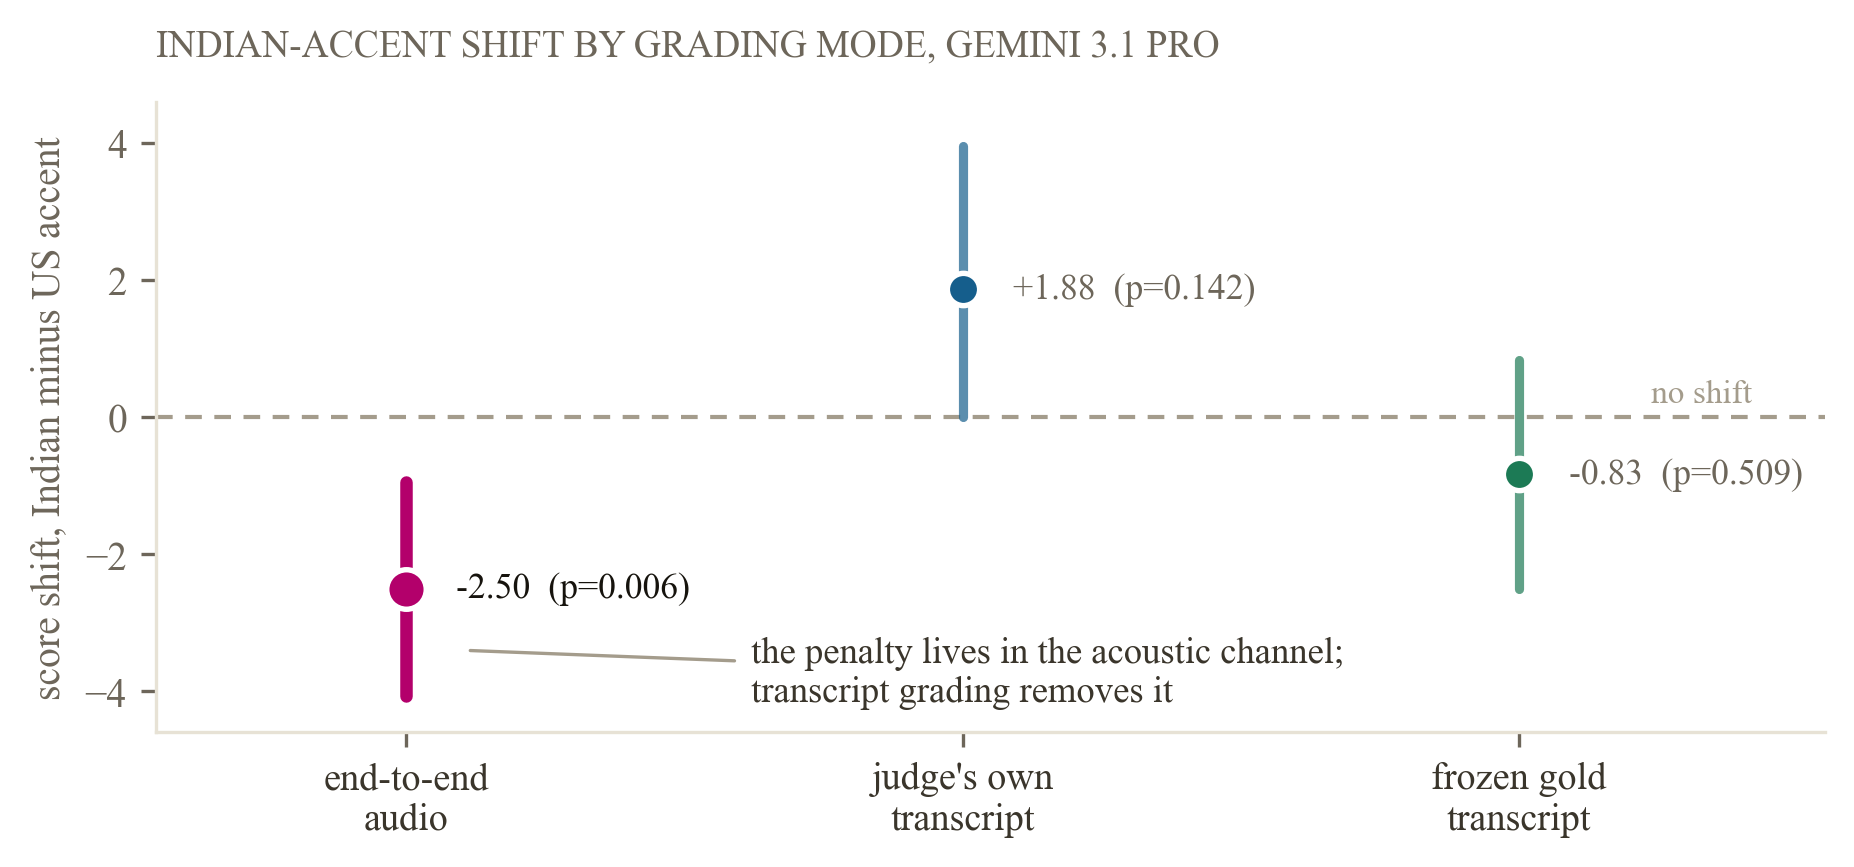
\includegraphics[width=\columnwidth]{assets/figure2_decomposition.png}
\caption{Gemini 3.1 Pro's Indian-accent shift on the original voice pair under three grading modes. The penalty is present only when the judge hears the audio.}
\label{fig:decomp}
\end{figure}

\subsection{Real Speech Shows Large, Consistent Penalties}
\label{sec:realspeech}

On the 240 real recordings, both Gemini judges penalise every non-native first language relative to gender-matched native speakers reading the same sentences (Tables~\ref{tab:l2arctic} and \ref{tab:l2ci}, Figure~\ref{fig:l2arctic}). Under Pro the shift runs from $-4.27$ (Hindi, $p=3\times10^{-4}$) to $-15.67$ (Mandarin, $p<10^{-4}$); under Flash from $-6.08$ to $-14.20$. All twelve Gemini cells have $p\le4\times10^{-4}$, with $n=32$ per cell from four speakers per language. The two judges agree on both size and order, with Hindi penalised least and Mandarin and Vietnamese most, which contrasts with their disagreement on the TTS arms. Qwen2-Audio, scoring the same clips, shifts by at most $-1.25$ (all n.s.), but it gives essentially every clip one of two scores (85 or 95), so its flatness is partly a property of its output scale.

The score distributions explain part of the difference between judges. Pro's real-speech scores have mean 85.8 (sd 12.2) over 13 distinct values and Flash's mean 86.0 (sd 13.1) over 12, so both use a wide part of the scale. Qwen2-Audio uses only 85 and 95, so it can show at most a coarse shift.

This arm's rubric scores the reading, and real L2 speech does differ in fluency. A penalty here therefore shows how strongly a judge responds to non-native delivery, not that it is biased against content. What the arm establishes is the size, the consistency across speakers within each language, and the agreement between two production judges, all of which the TTS effects lacked.

Across all 33 accent tests in the paper, Benjamini-Hochberg at $q=0.05$ keeps 16: the twelve real-speech Gemini cells, the single-voice Pro Indian cell, the single-voice Qwen2-Audio British and Nigerian cells, and the multi-voice Flash Nigerian cell (Appendix~\ref{app:bh}).

\begin{table}[t]
\small
\centering
\setlength{\tabcolsep}{4pt}
\begin{tabular}{lrrr}
\toprule
First language & Pro & Flash & Qwen2-Audio \\
\midrule
Hindi & $\mathbf{-4.27}$ & $\mathbf{-6.08}$ & $-0.31$ \\
Korean & $-7.08$ & $-8.14$ & $-0.62$ \\
Spanish & $-9.33$ & $-9.61$ & $-1.25$ \\
Arabic & $-13.08$ & $-13.02$ & $-0.62$ \\
Vietnamese & $-15.27$ & $-14.20$ & $-0.94$ \\
Mandarin & $-15.67$ & $-14.20$ & $-0.31$ \\
\midrule
Native mean (m / f) & 94.2 / 94.7 & 93.9 / 95.6 & 94.2 \\
\bottomrule
\end{tabular}
\caption{Real speech: shift against gender-matched native speakers, read-aloud rubric, $n=32$ per cell. Every Gemini cell has $p\le4\times10^{-4}$ and survives correction; no Qwen2-Audio cell is significant. Bold: smallest Gemini penalty per judge. Qwen2-Audio's native row is its overall mean, since it uses two score values.}
\label{tab:l2arctic}
\end{table}

\begin{figure}[t]
\centering
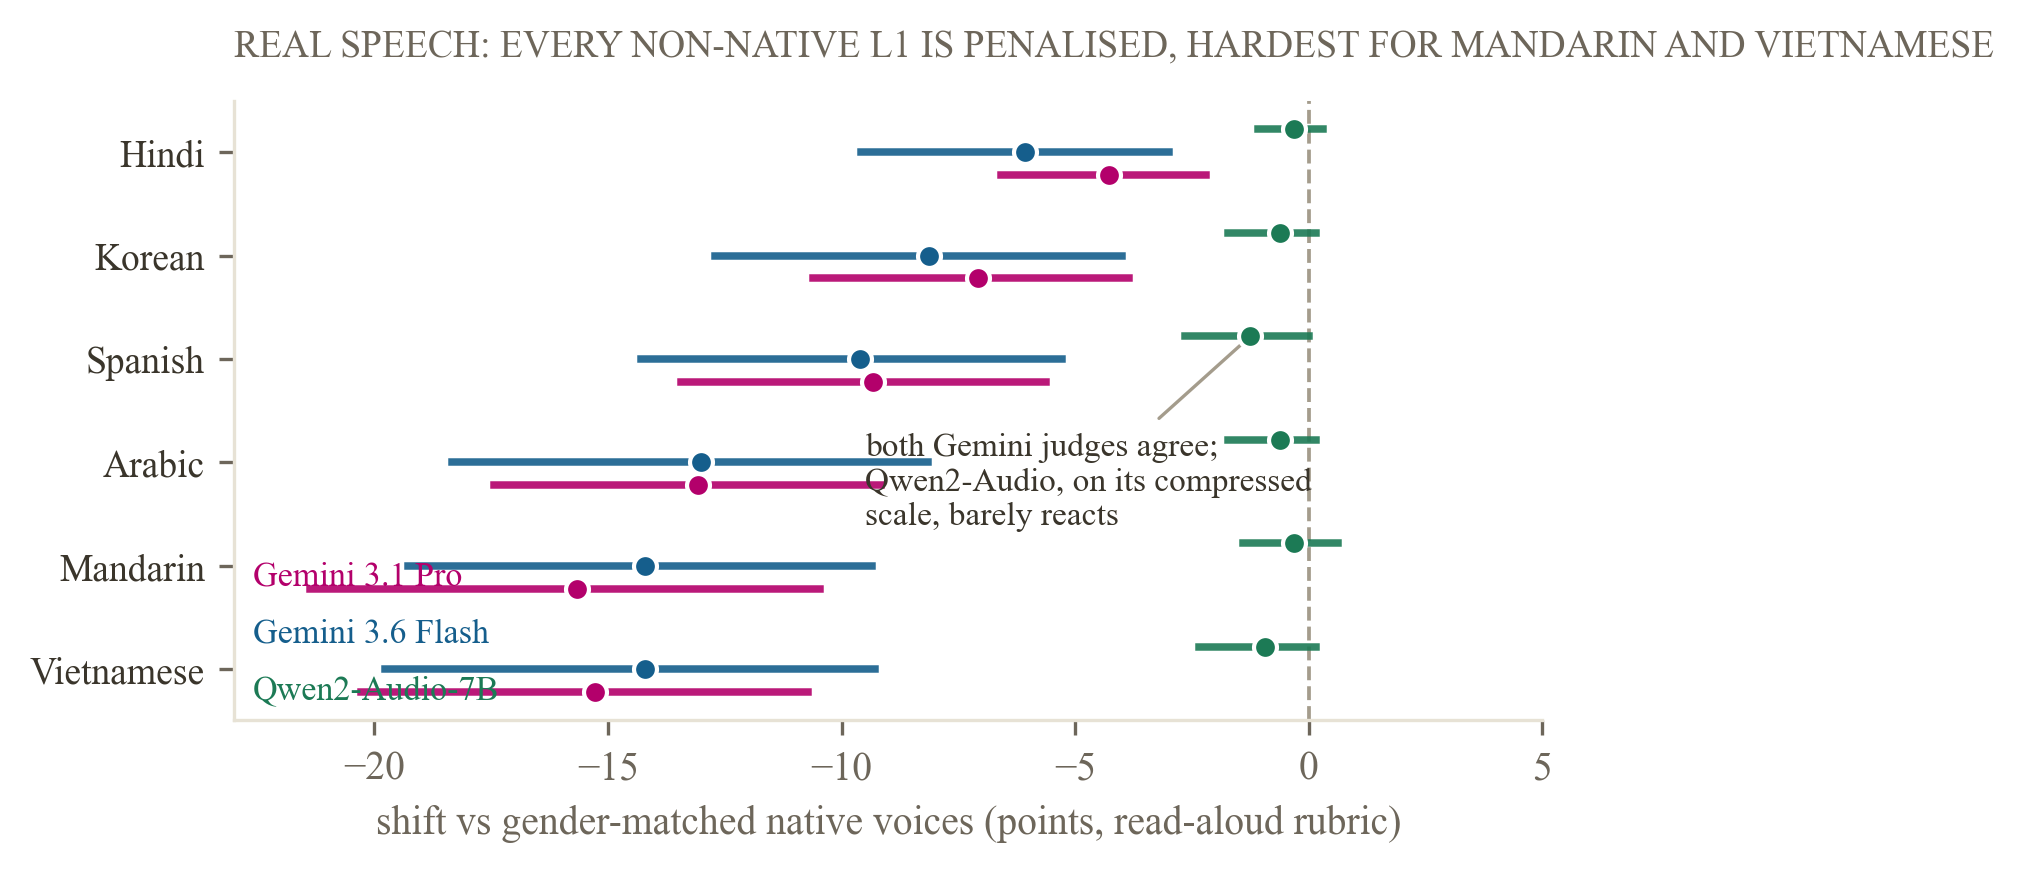
\includegraphics[width=\columnwidth]{assets/figure5_l2arctic.png}
\caption{Real speech: shift by first language against native speakers, with 95\% bootstrap intervals, $n=32$ per cell. Both Gemini judges agree on size and order; Qwen2-Audio barely moves on its two-value scale.}
\label{fig:l2arctic}
\end{figure}

\begin{table}[t]
\small
\centering
\setlength{\tabcolsep}{0.8pt}
\footnotesize
\begin{tabular}{lcc}
\toprule
L1 & Pro [95\% CI] & Flash [95\% CI] \\
\midrule
Arabic & $-13.08$ [$-17.45$, $-9.16$] & $-13.02$ [$-18.33$, $-8.16$] \\
Hindi & $-4.27$ [$-6.58$, $-2.20$] & $-6.08$ [$-9.58$, $-2.99$] \\
Korean & $-7.08$ [$-10.61$, $-3.85$] & $-8.14$ [$-12.72$, $-3.99$] \\
Mandarin & $-15.67$ [$-21.39$, $-10.47$] & $-14.20$ [$-19.28$, $-9.35$] \\
Spanish & $-9.33$ [$-13.43$, $-5.63$] & $-9.61$ [$-14.30$, $-5.29$] \\
Vietnamese & $-15.27$ [$-20.28$, $-10.73$] & $-14.20$ [$-19.78$, $-9.29$] \\
\bottomrule
\end{tabular}
\caption{Real-speech shifts with 95\% bootstrap intervals, $n=32$ per cell. Score distributions: Pro mean 85.8 (sd 12.2, 13 distinct values); Flash mean 86.0 (sd 13.1, 12 distinct values); Qwen2-Audio mean 94.2 (2 distinct values, 85 and 95).}
\label{tab:l2ci}
\end{table}

\subsection{Delivery Perturbations Are Null}
\label{sec:delivery}
None of the five delivery perturbations changed the score significantly under either Gemini judge or either prompt (all $p>0.1$, $|d_z|<0.36$, $n=21$ to 24 per cell; Figure~\ref{fig:delivery} and Table~\ref{tab:delivery}). The largest shift is Flash's $-3.70$ for filled pauses under the neutral rubric ($p=0.11$), which goes to $0.00$ under the ignore-delivery instruction. With 24 items, we read this as inconclusive, as our power planning expected for this secondary arm, and not as evidence that delivery never matters.

\begin{figure}[t]
\centering
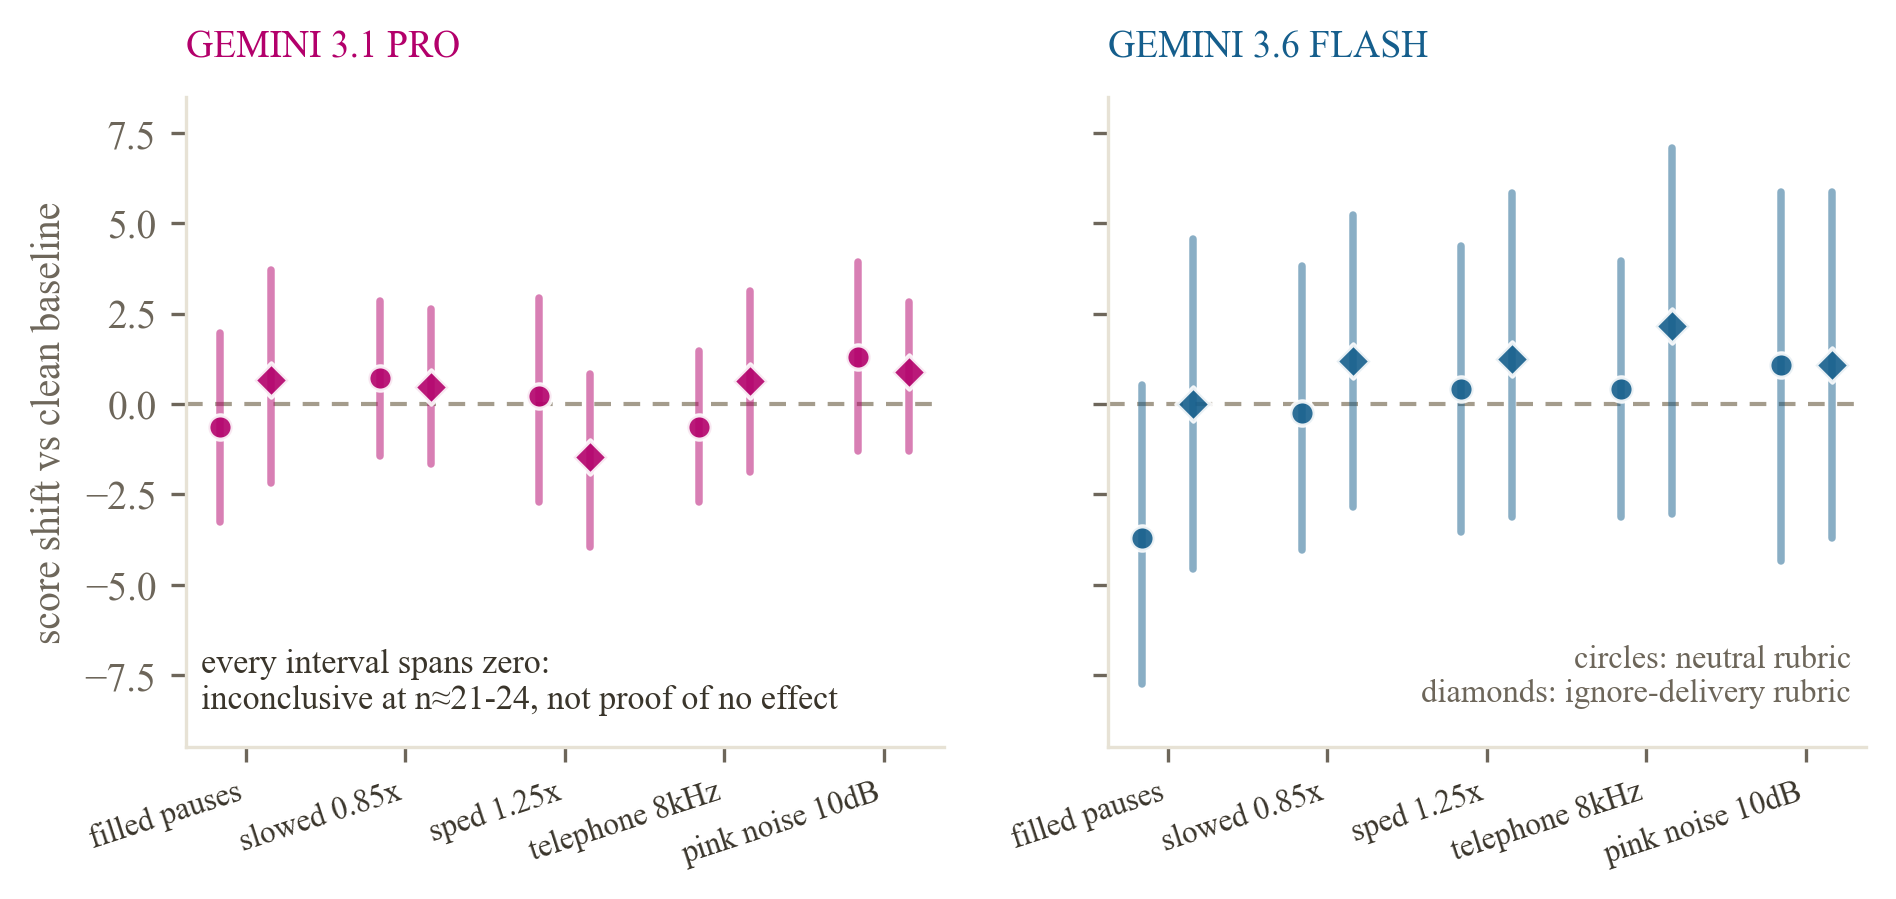
\includegraphics[width=\columnwidth]{assets/figure3_delivery.png}
\caption{Delivery perturbations, two judges and two prompts. Every 95\% interval spans zero ($n=21$ to 24 per cell).}
\label{fig:delivery}
\end{figure}

\begin{table*}[t]
\small
\centering
\begin{tabular}{llrcrrcr}
\toprule
 & & \multicolumn{3}{c}{Neutral rubric} & \multicolumn{3}{c}{Ignore-delivery rubric} \\
\cmidrule(lr){3-5}\cmidrule(lr){6-8}
Judge & Perturbation ($n$) & Shift & 95\% CI & $p$ & Shift & 95\% CI & $p$ \\
\midrule
Pro & filled pauses (23) & $-0.65$ & [$-3.26$, $+1.96$] & 0.76 & $+0.65$ & [$-2.17$, $+3.70$] & 0.78 \\
 & slowed 0.85$\times$ (21) & $+0.71$ & [$-1.43$, $+2.86$] & 0.69 & $+0.48$ & [$-1.67$, $+2.62$] & 0.83 \\
 & sped 1.25$\times$ (24) & $+0.21$ & [$-2.71$, $+2.92$] & 1.00 & $-1.46$ & [$-3.96$, $+0.83$] & 0.33 \\
 & telephone 8 kHz (24) & $-0.62$ & [$-2.71$, $+1.46$] & 0.71 & $+0.62$ & [$-1.88$, $+3.12$] & 0.75 \\
 & pink noise 10 dB (23) & $+1.30$ & [$-1.30$, $+3.91$] & 0.44 & $+0.87$ & [$-1.30$, $+2.83$] & 0.56 \\
\midrule
Flash & filled pauses (23) & $-3.70$ & [$-7.74$, $+0.52$] & 0.11 & $0.00$ & [$-4.57$, $+4.57$] & 1.00 \\
 & slowed 0.85$\times$ (21) & $-0.24$ & [$-4.05$, $+3.81$] & 1.00 & $+1.19$ & [$-2.86$, $+5.24$] & 0.65 \\
 & sped 1.25$\times$ (24) & $+0.42$ & [$-3.54$, $+4.38$] & 0.92 & $+1.25$ & [$-3.12$, $+5.83$] & 0.66 \\
 & telephone 8 kHz (24) & $+0.42$ & [$-3.12$, $+3.96$] & 0.92 & $+2.17$ & [$-3.04$, $+7.08$] & 0.46 \\
 & pink noise 10 dB (23) & $+1.09$ & [$-4.35$, $+5.87$] & 0.75 & $+1.09$ & [$-3.70$, $+5.87$] & 0.74 \\
\bottomrule
\end{tabular}
\caption{Delivery perturbations against the clean rendering of the same answer, one voice (American, female). No cell is significant.}
\label{tab:delivery}
\end{table*}

\subsection{Comparison with Prior Voice-Bias Results}
\label{sec:prior}

Table~\ref{tab:prior} places our arms next to published voice-bias studies. Studies that vary the voice with one synthetic voice per group find effects in some cells and not others \citep{satish2026thevoicebehi,wei2026biasintheear}, which is what our single-voice arm also produced. Our replication shows that such cells can belong to the chosen voice. Studies with real speakers find larger and more consistent effects \citep{koenecke2020racial,lin2026vibevoiceind}, as our real-speech arm does, but real speakers also differ in fluency and recording conditions, which a content-fixed TTS design avoids. Our results suggest using both: several synthetic voices per group for a clean content comparison, and real speakers to check the size of the effect.

\begin{table*}[t]
\small
\centering
\begin{tabular}{>{\raggedright\arraybackslash}p{4.0cm}>{\raggedright\arraybackslash}p{2.6cm}>{\raggedright\arraybackslash}p{3.6cm}>{\raggedright\arraybackslash}p{5.8cm}}
\toprule
Study & Model's role & Voice manipulation & Reported effect \\
\midrule
\citet{koenecke2020racial} & transcriber (5 ASR systems) & real speakers, Black vs white & WER 0.35 vs 0.19 \\
The Voice Behind the Words \citep{satish2026thevoicebehi} & respondent & voice cloning, 6 accents $\times$ 2 genders & lower helpfulness for Eastern European accents, mainly female voices \\
BiasInEar \citep{wei2026biasintheear} & test-taker (spoken MCQ) & synthetic voices, accents, languages & robust to demographic factors; sensitive to language and option order \\
VIBE \citep{lin2026vibevoiceind} & respondent (open-ended) & human-recorded speech & significant shifts from gender and accent cues \\
\citet{wang2026priorongevidence} & pronunciation feedback & L2-ARCTIC, 6 first languages & coherent reasoning for a wrong rating in 39.6\% of cells \\
\midrule
\textbf{This work, single voice} & grader & 1 TTS voice per gender, 4 accents & Pro, Indian: $-2.50$ ($p=0.005$) \\
\textbf{This work, six more voices} & grader & 6 TTS voices, same accents & Pro, Indian: $-0.76$ ($p=0.35$); voices $+2.08$ to $-4.58$ \\
\textbf{This work, real speech} & grader & L2-ARCTIC vs CMU ARCTIC & Gemini: $-4.3$ to $-15.7$ (all $p\le4\times10^{-4}$); Qwen2-Audio: $\le 1.25$ (n.s.) \\
\bottomrule
\end{tabular}
\caption{Our results next to published voice-bias studies. Effects are copied from each paper and use its own metric; ours are score shifts on a 100-point scale. Ours is the only study that puts the audio model in the grader role with the evaluee's voice as the treatment.}
\label{tab:prior}
\end{table*}

\subsection{Pre-registered Directions}
\label{sec:prereg}

Table~\ref{tab:prereg} scores the four directions. D1 looked confirmed in the single-voice arm, failed to replicate across voices, and holds strongly on real speech under a delivery rubric. D2 holds on the TTS arms, where the three judges disagree in sign, and reverses on real speech, where the two Gemini judges agree closely. D3 holds for the one voice-level penalty we found. D4 is not supported at this sample size.

\begin{table}[t]
\small
\centering
\begin{tabular}{>{\raggedright\arraybackslash}p{2.9cm}>{\raggedright\arraybackslash}p{4.6cm}}
\toprule
Direction & Outcome \\
\midrule
D1: L2 accents scored lower & TTS: one cell, did not replicate. \textbf{Real speech: holds} for both Gemini judges \\
D2: differs by family & \textbf{Holds} on TTS; reversed on real speech (Gemini judges agree) \\
D3: transcript removes effect & \textbf{Holds} for the original voice pair ($-6.04$, $p=4\times10^{-4}$) \\
D4: delivery leaks into content & Not supported (all $p>0.1$) \\
\bottomrule
\end{tabular}
\caption{Pre-registered directions and outcomes. Bold: supported.}
\label{tab:prereg}
\end{table}

\section{Discussion}
\label{sec:discussion}

\textbf{For people who audit audio judges.} A single-voice design produced a result that passed every check we would normally trust: a pre-registered direction, a significant test that survived correction, and a channel test locating the effect in the audio. It still turned out to be a property of one voice under one rubric. Audits should use several voices per accent or gender, report the spread across voices next to the mean, and treat the rubric's format as a design choice that can change the answer.

\textbf{Why one voice can mislead.} Under Pro, the Indian-minus-American shift ranges over 6.66 points across the seven voice sets we tested (the original pair and six new voices), from $+2.08$ to $-4.58$, while the pooled shift over the six new voices is $-0.76$. Flash's range is 6.84 points. Any single voice pair is therefore a draw from a wide distribution, and a draw near one end of it looks like an accent effect. With $n=48$ pairs, the single-voice test had enough power to make that draw significant. The fix is to treat the voice as a random factor: sample several voices per group and test the accent effect against the variation between voices, not only against the variation between items.

\textbf{For people who deploy audio judges.} On real speech, two production judges score non-native readings 4 to 16 points lower, with the same ordering across first languages. Under a delivery rubric some of this may be legitimate, since L2 speech differs in fluency. Under a content rubric it would not be. We have not shown which part is which, so anyone who uses an audio judge for L2 speakers should compare its scores with human ratings of the same recordings before relying on them. Transcript-first grading removes the audio channel entirely. That is a useful mitigation when the task is about content, and a loss when delivery is part of what is being assessed.

\section{Conclusion}

We held the words fixed and changed only the voice to see whether audio judges score the speaker. A single-voice TTS audit found a significant Indian-accent penalty under Gemini 3.1 Pro that lived in the audio channel. Six more voices and a four-part rubric removed it, so we report our own headline as a replication failure. On real non-native speech, both Gemini judges penalised every first language we tested by 4 to 16 points, consistently and in the same order, while Qwen2-Audio barely moved. Measured voice bias depends on the voices sampled, the rubric and the judge family, and a design that fixes all three may say more about the design than about the model.

\textbf{Future work.} Three extensions follow directly. First, collect human ratings of the 240 real-speech clips under the same rubric, to separate legitimate fluency differences from judge bias. Second, use a real-speech corpus in which speakers give content-bearing answers, so a content rubric can be applied to real voices. Third, add a frontier non-Google audio judge and more items per arm, to test whether the multi-voice instability and the delivery nulls hold with more power.

\section*{Limitations}

\textbf{The rubrics differ across arms.} The TTS arms score content; the real-speech arm scores the reading, because ARCTIC sentences carry no answer content. The real-speech penalties are about delivery, and their size should not be read as content bias.

\textbf{Recording conditions differ with nativeness.} The native CMU ARCTIC voices are studio recordings of experienced voice talent; the L2-ARCTIC speakers are not professional narrators. Part of the per-language gradient may come from recording quality and speaking experience rather than accent. Four speakers per language also limits how far the results generalise, although the effects are consistent across speakers and across two judges.

\textbf{Sample size.} The TTS arms use 24 items, and the multi-voice arm 12 of them, under a small compute budget. The delivery nulls and the non-significant multi-voice cells may be underpowered.

\textbf{Uneven judge coverage.} Both Gemini judges scored every arm except the decomposed rubric, which only Pro scored. Qwen2-Audio scored only the single-voice and real-speech arms, and its two-to-four-value output scale limits what its null results show. No frontier non-Google audio judge was tested.

\textbf{Manipulation check.} The accent check used a Gemini classifier on Gemini-generated audio; no independent or human check was run. The multi-voice result reduces how much this matters, since no accent claim rests on the TTS arm.

\textbf{Noise proxy.} Pink noise at a measured SNR stands in for multi-talker babble.

\section*{Ethical Considerations}
This study measures whether automated graders treat speakers differently by accent and first language, with the goal of protecting the people who are graded. The real-speech arm uses L2-ARCTIC, a research corpus released under CC BY-NC 4.0, and the freely available CMU ARCTIC voices. We release per-clip scores and selection metadata but do not redistribute the recordings. The TTS voices are prebuilt synthetic voices and imitate no real person. We use accent and first-language labels only as experimental conditions and make no claims about the speakers themselves. Our negative replication is a warning against citing single-voice audit results as evidence for or against bias in deployed systems.

\section*{Use of AI Assistants}
\textbf{In the experiments:} Gemini 3.1 Pro, Gemini 3.6 Flash and Qwen2-Audio-7B-Instruct are the judges under study. Gemini 3.5 Flash wrote the answer bank, Gemini 3.1 Flash TTS produced all synthetic speech, and Gemini 3.6 Flash ran the accent manipulation check and the word-error-rate gate, and its transcripts were used in the own-transcript mode. \textbf{Code and setup:} an AI coding assistant (Claude) helped write the generation, judging and analysis scripts; every script was run and its outputs checked by the authors. \textbf{Figures:} Figure~\ref{fig:schematic} was generated with Nano Banana 2 (Gemini 3.1 Flash Image) from a written description of the design, and every label was checked by hand; the data figures were drawn with matplotlib from the analysis output. \textbf{Writing:} Claude helped draft and edit the text, and the authors revised every section. All design decisions, statistical choices and claims are the authors', and every number was checked against the scripted analysis output.
